\appendix
\newpage
\section{Surrogate data example} \label{appendix:surrogate-example}

\begin{figure}[h]
\begin{center}
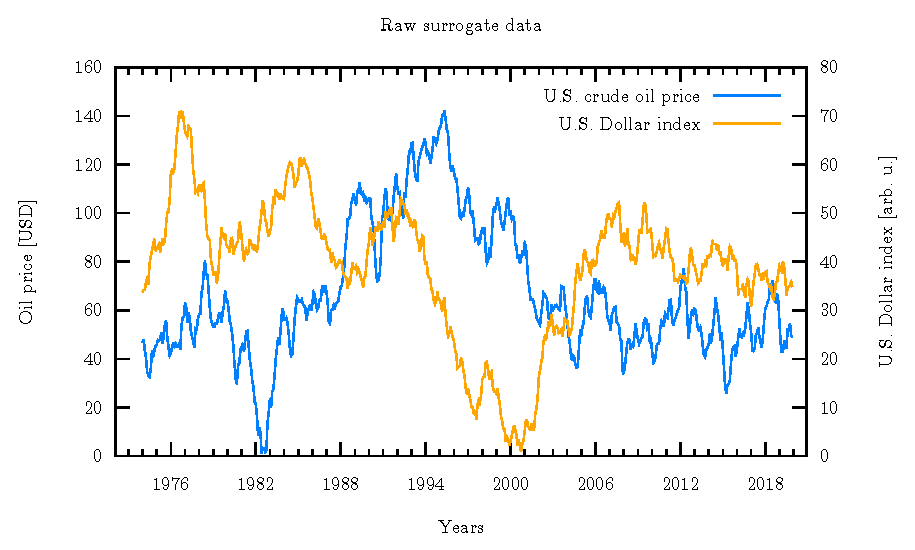
\includegraphics[width=0.8\textwidth]{./code/plot/surrogate_raw.eps}
\caption{Plot of raw surrogate data of crude oil price and U.S. Dollar Index.}
\label{fig:s-raw}
\end{center}
\end{figure}

\begin{figure}[h]
\begin{center}
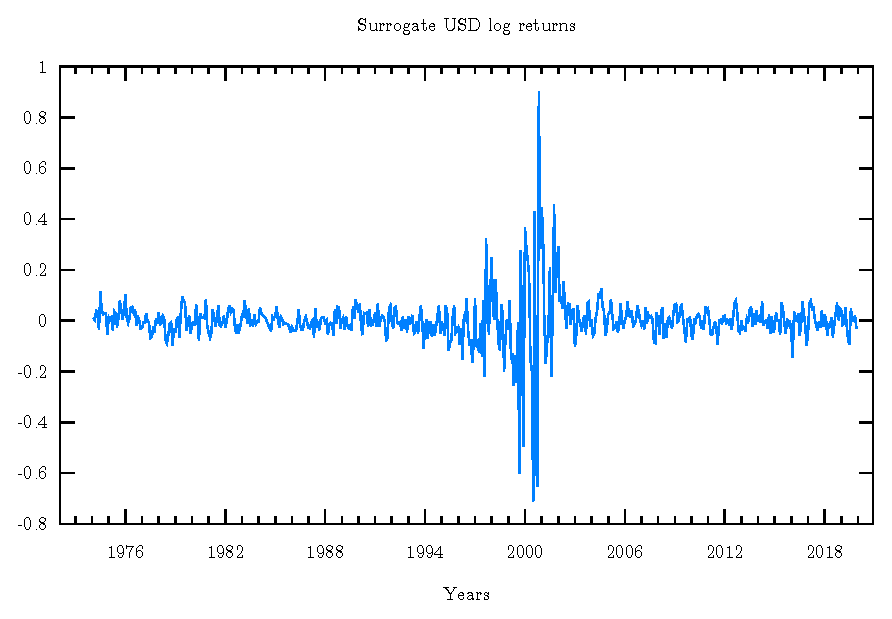
\includegraphics[width=0.8\textwidth]{./code/plot/surrogate_dollar_logret.eps}
\caption{Plot of a surrogate data generated from U.S. Dollar Index log returns.}
\label{fig:s-usd-logret}
\end{center}
\end{figure}

\begin{figure}
\begin{center}
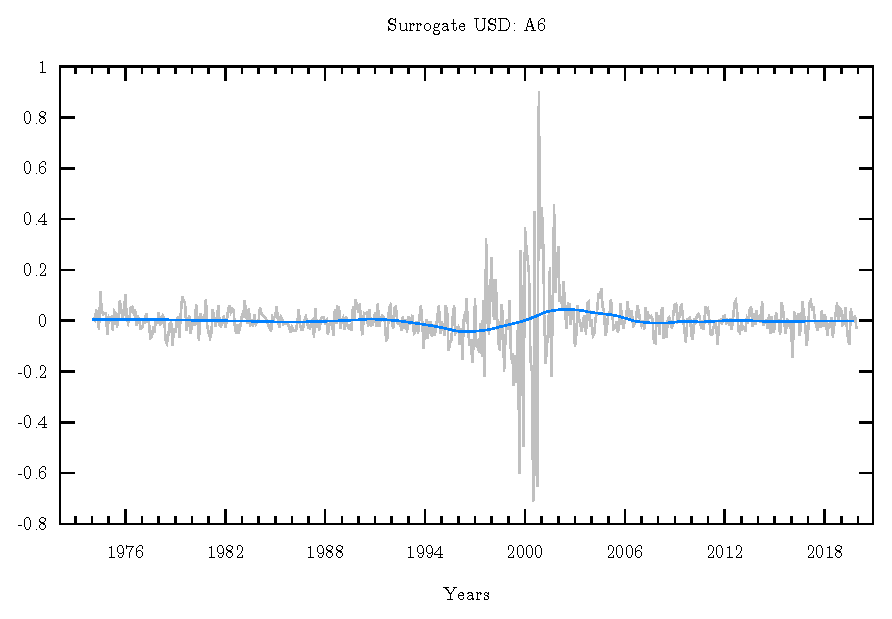
\includegraphics[width=0.8\textwidth]{./code/plot/surrogate_usd_wr_A6.eps}
\caption{Plot of A6 component of wavelet decomposition of surrogate U.S. Dollar Index log returns. 
	Plot of the surrogate log returns in grey. A6 scale corresponds to $>$128 months.}
\end{center}
\label{fig:s-usd-wr-a6}
\end{figure}

\begin{figure}
\begin{center}
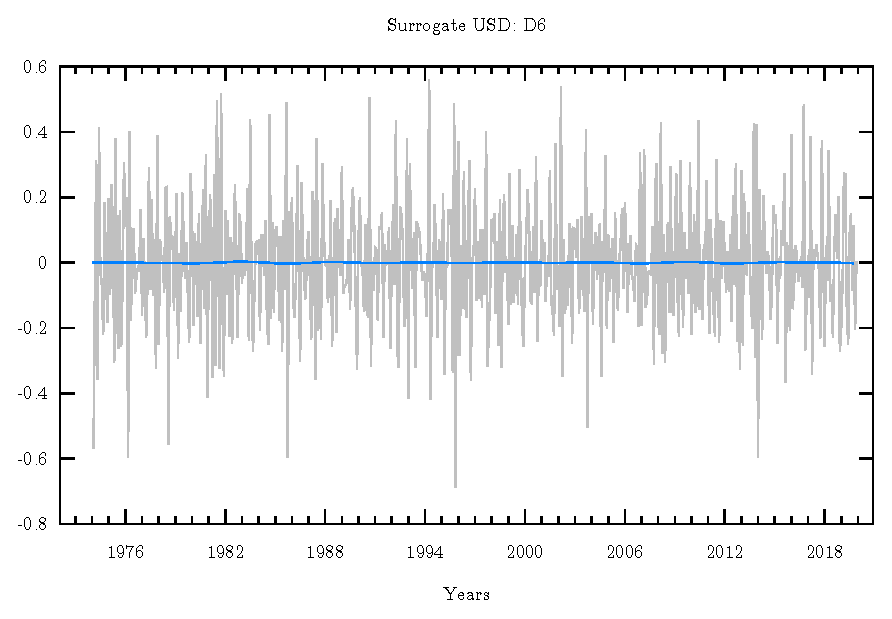
\includegraphics[width=0.8\textwidth]{./code/plot/surrogate_usd_wr_D6.eps}
\caption{Plot of D6 component of wavelet decomposition of surrogate U.S. Dollar Index log returns. 
	Plot of the surrogate log returns in grey. D6 scale corresponds to 64-128 months.}
\end{center}
\label{fig:s-usd-wr-d6}
\end{figure}

\begin{figure}
\begin{center}
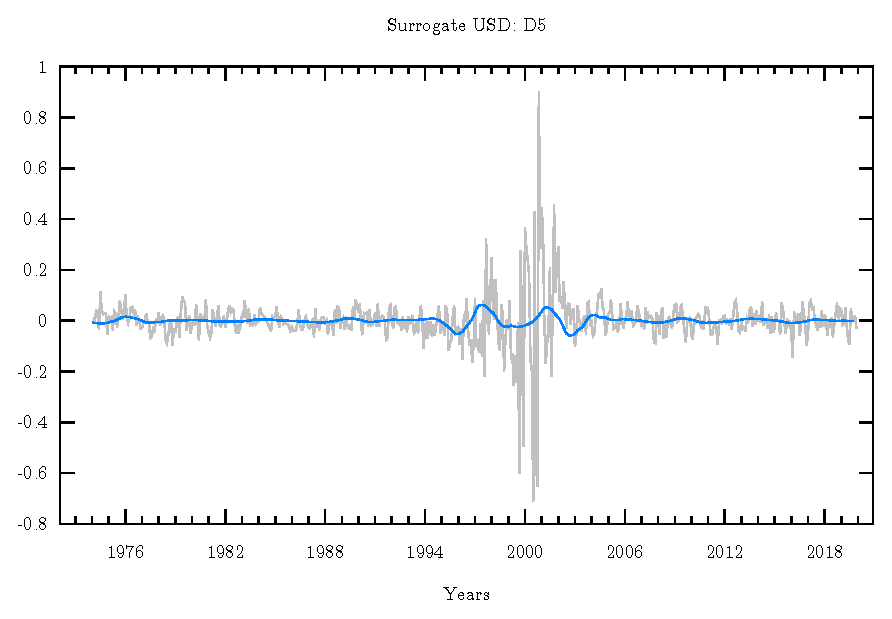
\includegraphics[width=0.8\textwidth]{./code/plot/surrogate_usd_wr_D5.eps}
\caption{Plot of D5 component of wavelet decomposition of surrogate U.S. Dollar Index log returns. 
	Plot of the surrogate log returns in grey. D5 scale corresponds to 32-64 months.}
\end{center}
\label{fig:s-usd-wr-d5}
\end{figure}

\begin{figure}
\begin{center}
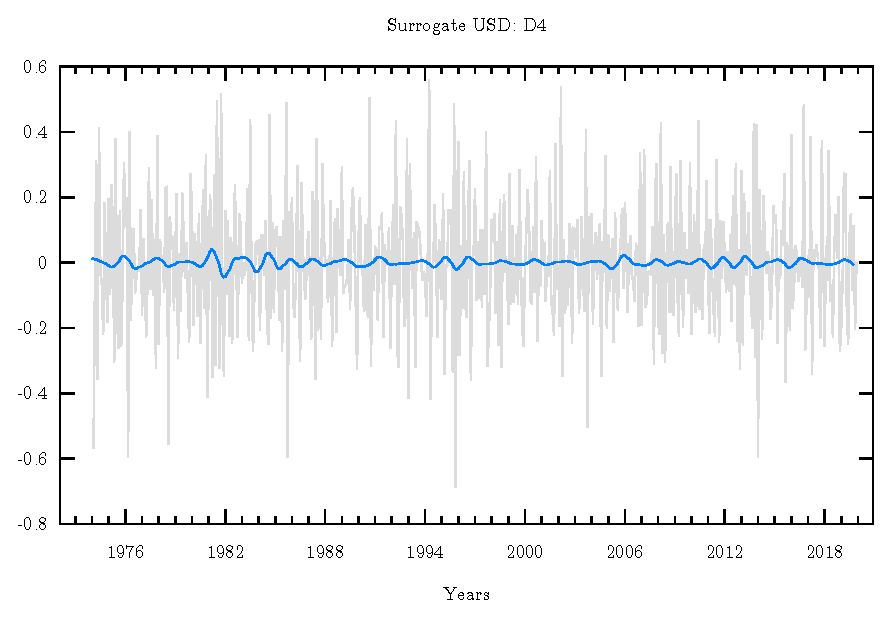
\includegraphics[width=0.8\textwidth]{./code/plot/surrogate_usd_wr_D4.eps}
\caption{Plot of D4 component of wavelet decomposition of surrogate U.S. Dollar Index log returns. 
	Plot of the surrogate log returns in grey. D4 scale corresponds to 16-32 months.}
\end{center}
\label{fig:s-usd-wr-d4}
\end{figure}

\begin{figure}
\begin{center}
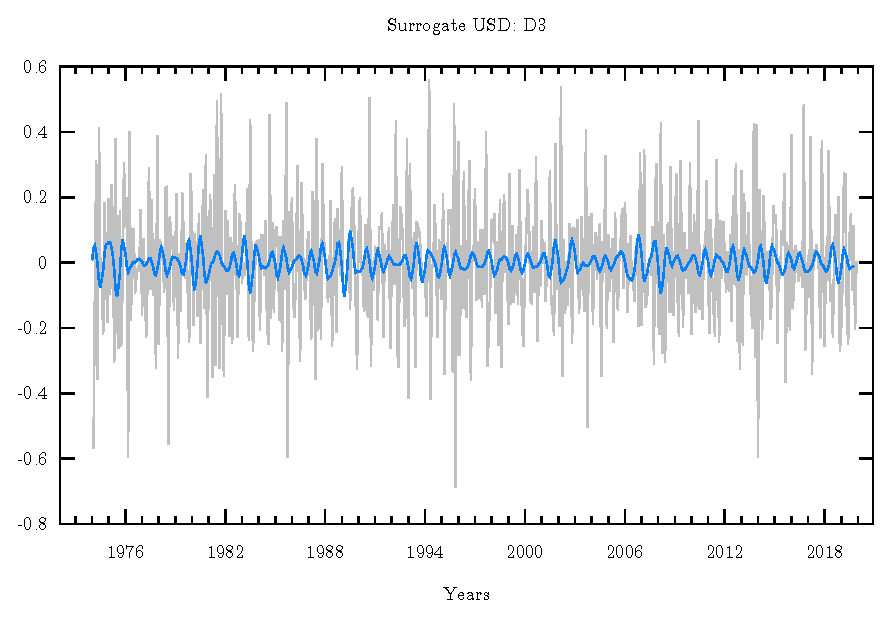
\includegraphics[width=0.8\textwidth]{./code/plot/surrogate_usd_wr_D3.eps}
\caption{Plot of D3 component of wavelet decomposition of surrogate U.S. Dollar Index log returns. 
	Plot of the surrogate log returns in grey. D3 scale corresponds to 8-16 months.}
\end{center}
\label{fig:s-usd-wr-d3}
\end{figure}

\begin{figure}
\begin{center}
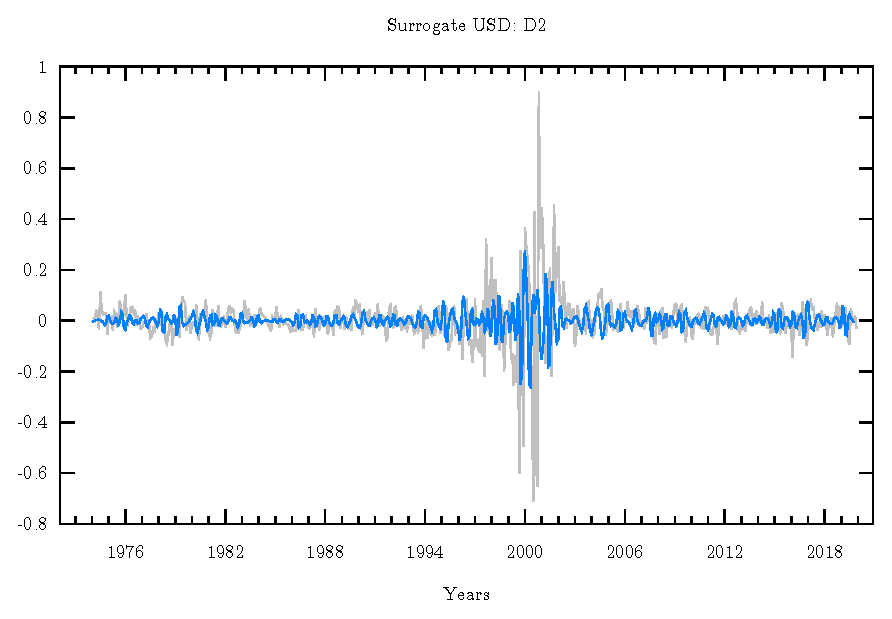
\includegraphics[width=0.8\textwidth]{./code/plot/surrogate_usd_wr_D2.eps}
\caption{Plot of D2 component of wavelet decomposition of surrogate U.S. Dollar Index log returns. 
	Plot of the surrogate log returns in grey. D2 scale corresponds to 4-8 months.}
\end{center}
\label{fig:s-usd-wr-d2}
\end{figure}

\begin{figure}
\begin{center}
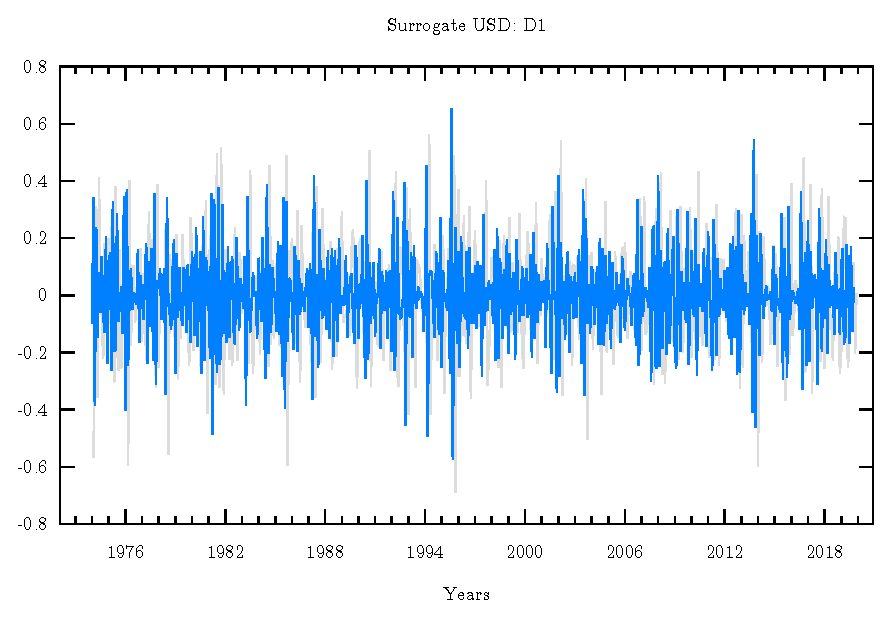
\includegraphics[width=0.8\textwidth]{./code/plot/surrogate_usd_wr_D1.eps}
\caption{Plot of D1 component of wavelet decomposition of surrogate U.S. Dollar Index log returns. 
	Plot of the surrogate log returns in grey. D1 scale corresponds to 2-4 months.}
\end{center}
\label{fig:s-usd-wr-d1}
\end{figure}

\begin{figure}
\begin{center}
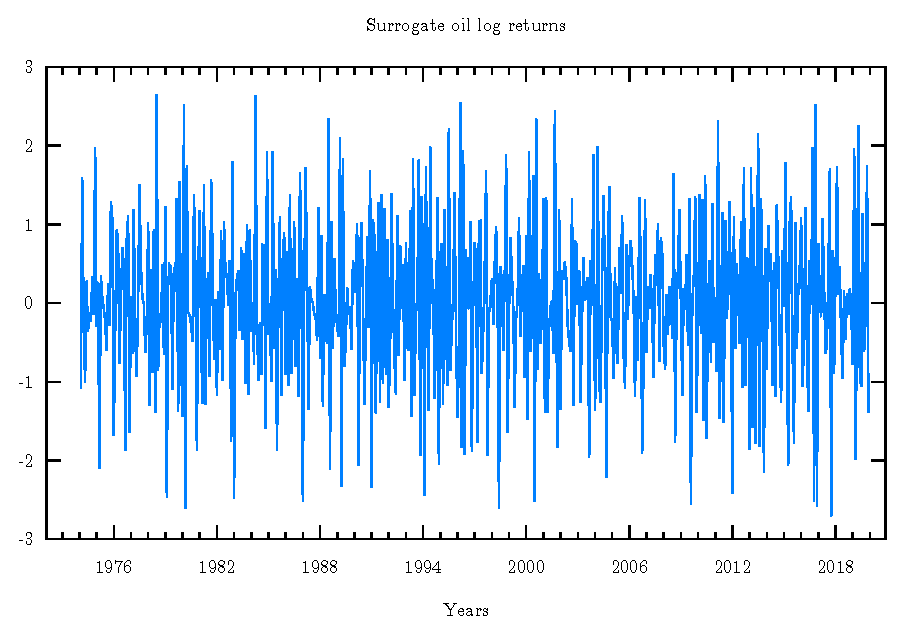
\includegraphics[width=0.8\textwidth]{./code/plot/surrogate_oil_logret.eps}
\caption{Plot of a surrogate data generated from oil price log returns.}
\label{fig:s-oil-logret}
\end{center}
\end{figure}


\begin{figure}
\begin{center}
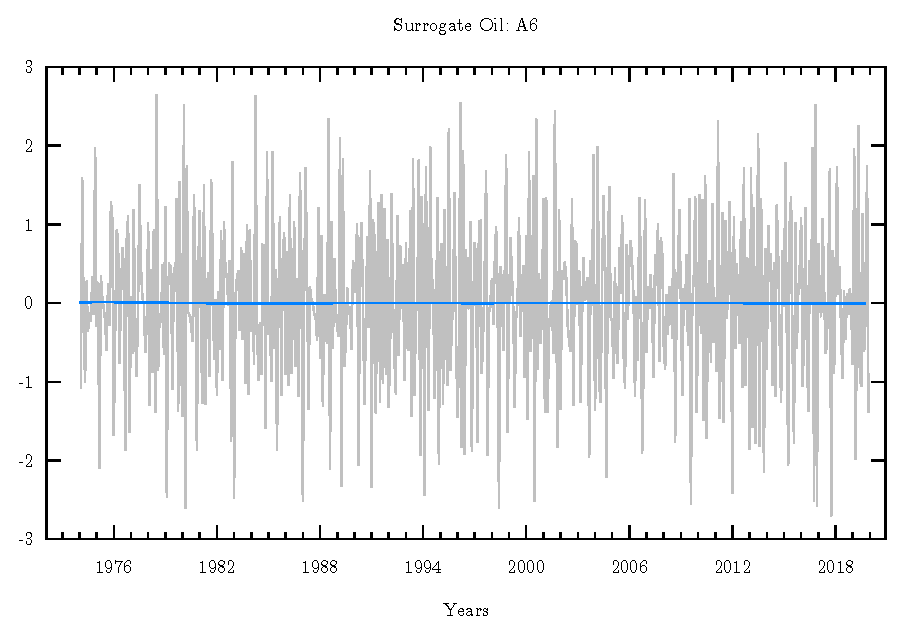
\includegraphics[width=0.8\textwidth]{./code/plot/surrogate_oil_wr_A6.eps}
\caption{Plot of A6 component of wavelet decomposition of surrogate oil price log returns. 
	Plot of the surrogate log returns in grey. A6 scale corresponds to $>$128 months.}
\end{center}
\label{fig:s-oil-wr-a6}
\end{figure}

\begin{figure}
\begin{center}
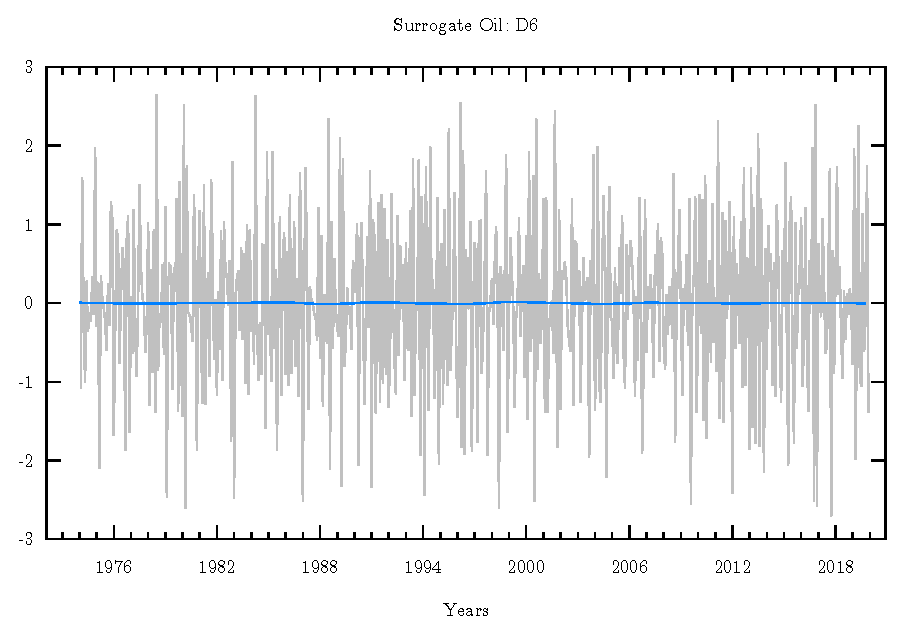
\includegraphics[width=0.8\textwidth]{./code/plot/surrogate_oil_wr_D6.eps}
\caption{Plot of D6 component of wavelet decomposition of surrogate oil price log returns. 
	Plot of the surrogate log returns in grey. D6 scale corresponds to 64-128 months.}
\end{center}
\label{fig:s-oil-wr-d6}
\end{figure}

\begin{figure}
\begin{center}
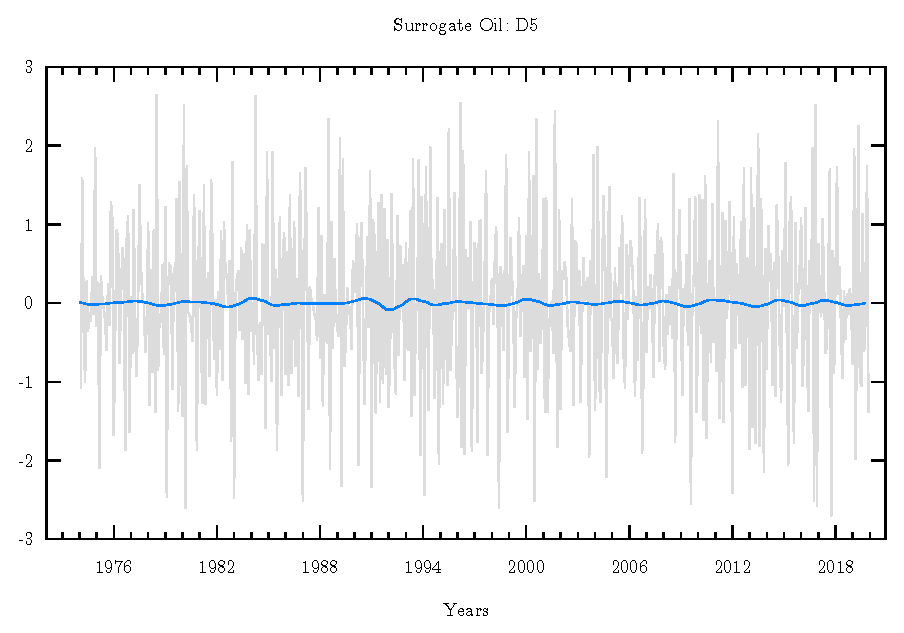
\includegraphics[width=0.8\textwidth]{./code/plot/surrogate_oil_wr_D5.eps}
\caption{Plot of D5 component of wavelet decomposition of surrogate oil price log returns. 
	Plot of the surrogate log returns in grey. D5 scale corresponds to 32-64 months.}
\end{center}
\label{fig:s-oil-wr-d5}
\end{figure}

\begin{figure}
\begin{center}
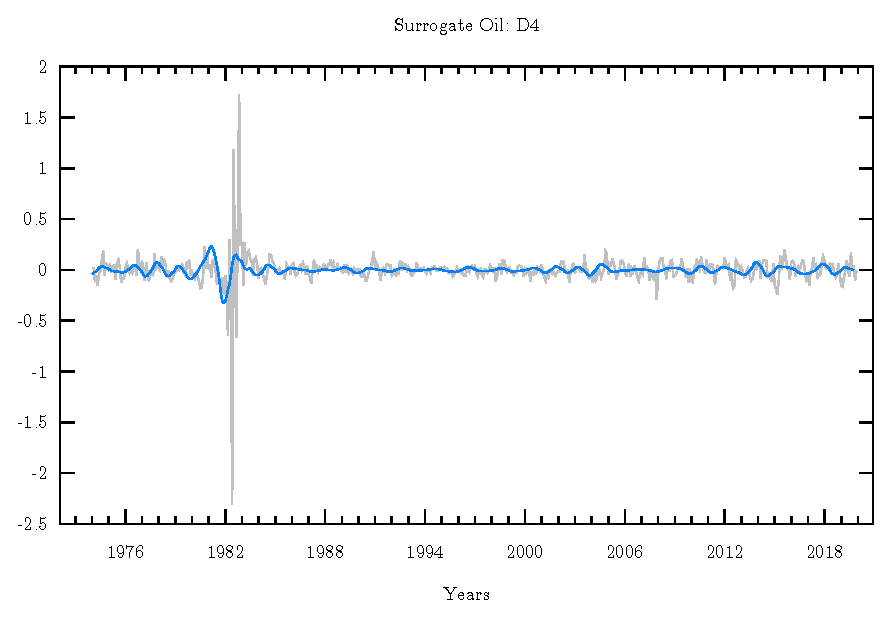
\includegraphics[width=0.8\textwidth]{./code/plot/surrogate_oil_wr_D4.eps}
\caption{Plot of D4 component of wavelet decomposition of surrogate oil price log returns. 
	Plot of the surrogate log returns in grey. D4 scale corresponds to 16-32 months.}
\end{center}
\label{fig:s-oil-wr-d4}
\end{figure}

\begin{figure}
\begin{center}
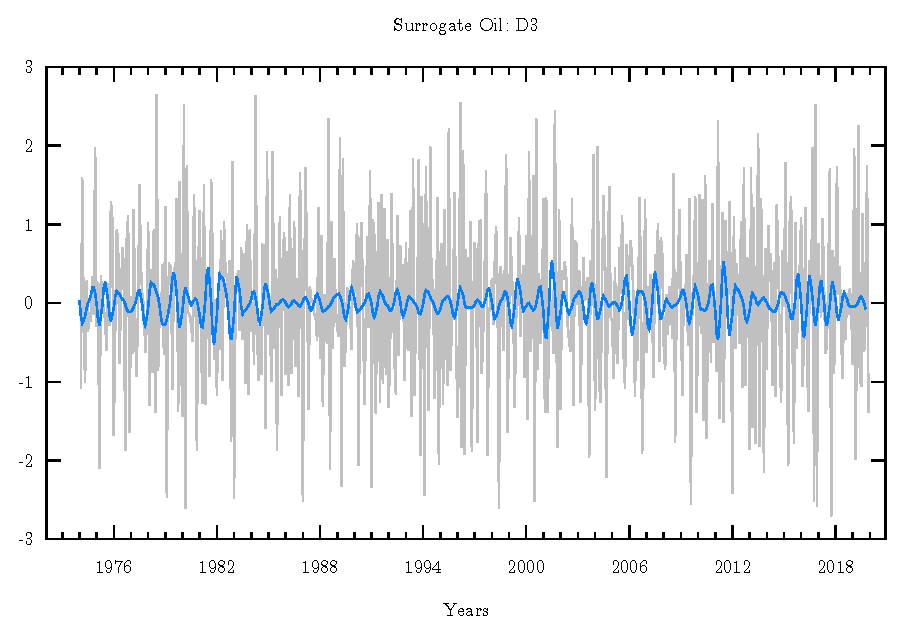
\includegraphics[width=0.8\textwidth]{./code/plot/surrogate_oil_wr_D3.eps}
\caption{Plot of D3 component of wavelet decomposition of surrogate oil price log returns. 
	Plot of the surrogate log returns in grey. D3 scale corresponds to 8-16 months.}
\end{center}
\label{fig:s-oil-wr-d3}
\end{figure}

\begin{figure}
\begin{center}
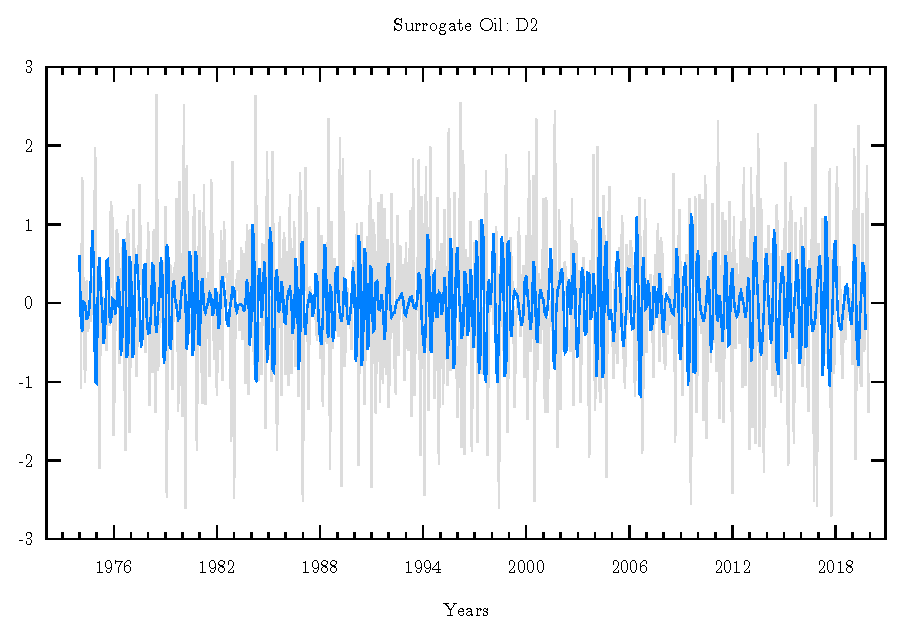
\includegraphics[width=0.8\textwidth]{./code/plot/surrogate_oil_wr_D2.eps}
\caption{Plot of D2 component of wavelet decomposition of surrogate oil price log returns. 
	Plot of the surrogate log returns in grey. D2 scale corresponds to 4-8 months.}
\end{center}
\label{fig:s-oil-wr-d2}
\end{figure}

\begin{figure}
\begin{center}
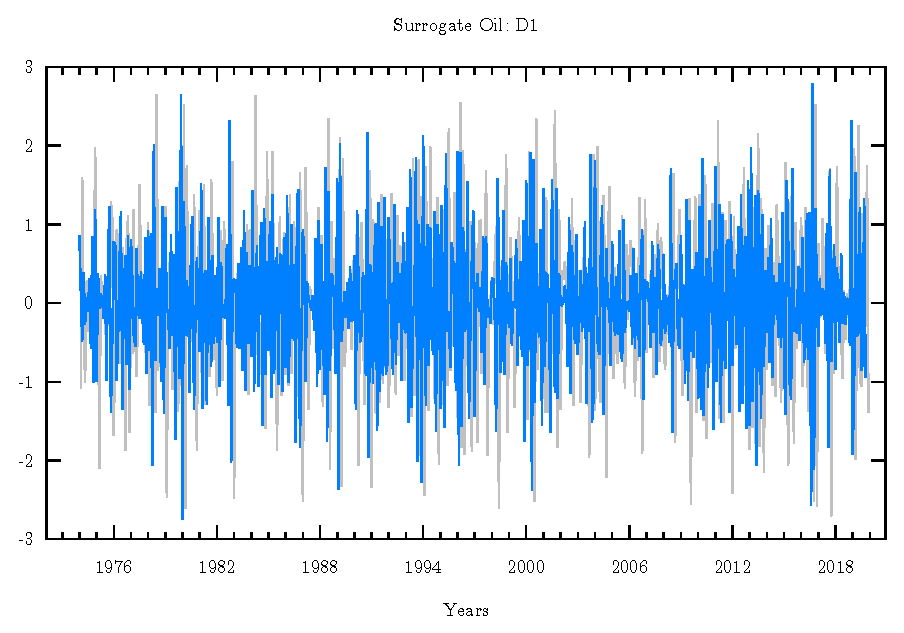
\includegraphics[width=0.8\textwidth]{./code/plot/surrogate_oil_wr_D1.eps}
\caption{Plot of D1 component of wavelet decomposition of surrogate oil price log returns. 
	Plot of the surrogate log returns in grey. D1 scale corresponds to 2-4 months.}
\end{center}
\label{fig:s-oil-wr-d1}
\end{figure}
